%!TEX root=Principal.tex
\chapter{MÉTODO CENTRADO NO USUÁRIO PARA PROJETOS DE INTERAÇÃO HUMANO-ROBÔ}
\label{cap:projetoihr}
Esse capítulo é dedicado a apresentação do método centrado no usuário para construção de robôs autônomos  que serão utilizados em tarefas de interação com seres humanos. Primeiro passo realizado foi a definição das fases necessárias para construir um projeto de interação entre humanos e robôs, de acordo com os estudos realizados sobre os modelos de processos de desenvolvimento de \emph{software}. Entre os modelos apresentados na literatura, existem duas grandes categorias dentre os modelos, são elas: os prescritivos ou tradicionais e os métodos ágeis.

A primeira categoria, os modelos prescritivos, tem como principal característica a definição de limites claros entre as fases do projeto. O foco dos modelos prescritivos está em grande parte na documentação presente em todas as fases do processo, e não apenas no código-fonte do sistema. Dentre os modelos prescritivos existem dois modelos que são base para os demais, modelo cascata e o modelo espiral~\cite{sommerville:2008, wazlawick:2013}.

O modelo cascata tem como maior característica a execução das tarefas de maneira sequencial, onde cada tarefa está contida em fases. Cada fase do processo possui o escopo bem definido. Este modelo foi utilizado por muito tempo, porém ele não tinha uma realimentação no processo de maneira que qualquer evolução deve ser tratada como um novo projeto. Com essa característica, algumas variações foram apresentadas para mitigar esse problema, como o cascata em V, em W e o em subprojetos~\cite{wazlawick:2013}. A documentação gerada no modelo cascata tem o objetivo de retratar o código produzido pela equipe de desenvolvimento, de maneira mais abstrata possibilitando um melhor entendimento do projeto por todos envolvidos.

Como uma evolução do modelo cascata e suas variações, surgiu o modelo espiral. Sua principal característica é a prototipação segmentada e cíclica. Esse ponto auxilia na mitigação dos riscos envolvendo o negócio do projeto. O trabalho com ciclos de interação é positivo, pois possibilita a documentação da evolução do projeto. O histórico de evolução é importante para identificar tomadas de decisões de problemas recorrentes e possíveis criações de padrões de projetos.

A segunda categoria dos modelos de processo de software, os modelos ágeis, tem como principal objetivo diminuir as definições das atividades e trabalhar de forma mais prática. Esse modelo é voltado a fatores humanos do desenvolvimento. Isso não quer dizer que os métodos ágeis sejam desprendidos de documentação ou que sejam simples demais. O principal ponto destes métodos é focar nos resultados e não no processo formal como um todo~\cite{sommerville:2008}.

Dentre os modelos ágeis, os mais conhecidos são o SCRUM e o XP (\textit{eXtreme Programming}). O SCRUM é uma metodologia focada na gestão de projetos. O objetivo é dividir o projeto em pequenos grupos de entregas chamados de \textit{sprints}, ou seja, corridas rápidas de desenvolvimento. Cada \textit{sprint} tem duração de 2 a 4 semanas, entre valores mínimo e máximo. Ele é recomendado para grandes projetos e com uma equipe bem inflada. Dessa forma, é possível ter um controle e indicadores de evolução do projeto de maneira mais rápida. Isso possibilita que mudanças de negócios e riscos sejam detectados e mitigados em um prazo menor~\cite{sutherland:2016}. O SCRUM ele segue uma linha de raciocínio parecida com o modelo espiral, porém o prazo entre os ciclos são pré determinado através dos \textit{sprints}.

O XP é um modelo ágil mais indicado à equipe de desenvolvimento. Ele é baseado em valores, princípios e regras. Por ser um modelo mais simples, ele é recomendado a equipes de pequeno e médio porte. Os princípios trabalhos dentro do XP são: simplicidade, respeito, comunicação, \textit{feedback} e coragem. Por ser um modelo voltado a equipe de desenvolvimento, não existe uma forma para condução do projeto como um todo. O objetivo é direcionar a equipe com boas práticas na condução do trabalho. Além do SCRUM e o XP, existem outros modelos ágeis, como o Lean , Crystal e o \textit{Feature Driven Development} (FDD)~\cite{wazlawick:2013}.

O uso de modelos ágeis é interessante quando o projeto possui mudanças de negócios com uma frequência mais elevada, dentro de um curto espaço temporal. Nesta tese é fundamental adotar um modelo de desenvolvimento de \textit{software}, pois fica mais claro identificar as fases de cada parte do projeto de interação humano-robô, além de deixar mapeado os passos necessários para evolução do projeto~\cite{sommerville:2008, wazlawick:2013}.

O modelo de negócio aplicado a robótica de serviços em um âmbito geral, é voltado mais a pesquisa do que o mercado propriamente. Sendo assim, é importante que o método para projetos em interação humano-robô possua iterações cíclicas onde seja contemplado sua evolução. Entretanto, o uso de metodologias ágeis não é recomendado, pois é necessário um amadurecimento de documentação e estrutura do projeto, que as metodologias ágeis não possuem uma boa governança. Nesse caso, o modelo de processo de \textit{software} mais indicado é o modelo espiral, pois atende os quesitos de documentação necessários e também possui a vantagem de ser iterativo. Dessa maneira, cada ciclo do projeto, pode ser considerado um novo versionamento do projeto de interação humano-robô.

É proposto nesta tese, um modelo espiral que contempla 4 fases: concepção, construção, teste e análise. Esse modelo proposto com base no modelo de processo tradicional espiral~\cite{sommerville:2008} é ilustrado através da figura~\ref{fig:espiral}.

\begin{figure}[ht!]
	\centering
	\begin{minipage}{0.7\textwidth}
		\caption{Modelo de processo para IHR proposto nesta tese com base no modelo espiral.}
		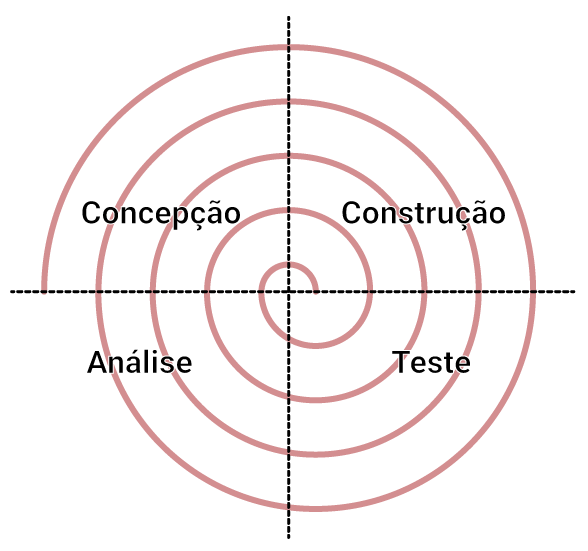
\includegraphics[width=\textwidth]{espiral_4_fases.png}
		\smallcaption{Fonte: o autor.}
		\label{fig:espiral}
	\end{minipage}
\end{figure}

Na fase de concepção é realizado o levantamento inicial das necessidades do projeto. Nesse levantamento todas as definições e contextualizações são realizadas. As definições de escopo, variáveis de observação, contexto de uso, questionário pré e pós teste, perfil do grupo de usuários pra execução dos testes, funcionalidades do robô, sensoriamento e atuadores, cenário de teste e submissão do projeto ao comitê de ética. 

A próxima fase é a da construção, nela é realizado algumas definições mais técnicas do robô como arquitetura de \textit{software} e construção física do robô, e a implementação dos mecanismos de decisão e controle do robô. Além disso, nessa fase são realizados alguns testes pilotos para obter as características dos perfis do publico alvo. Com essas informações podem ser trabalhadas as Personas que servirão de base para o projeto. Com base nas Personas, ajustes devem ser realizados para atender melhor as expectativas dos usuários durante a interação com o robô. A interação deve ser de maneira totalmente autônoma, pois deixará o resultado dos testes mais naturais e reais ao cenário.

Como apresentado na figura~\ref{fig:espiral} a sequência do projeto é a bateria de testes realizadas com os usuários diferentes dos testes piloto. Nessa fase o mais importante é realizar a coleta de informações que são utilizadas na fase de análises. A fase de análise é a última fase do ciclo do modelo de desenvolvimento de um projeto de robô autônomo que interage com humanos. Nela deve-se rodar testes estatísticos à fins de validar hipóteses nulas levantadas na definição do escopo. Além disso, discussões com bases em resultados qualitativos também são realizados. Eles auxiliam na definição e nos procedimentos que deverão ser executados na próxima iteração do modelo espiral. Uma visão geral do ciclo proposto nesta tese é apresentada através da figura~\ref{fig:pool}.


\begin{figure}[ht!]
	\centering
	\begin{minipage}{\textwidth}
		\caption{Detalhamento do processo apresentado no método proposto por essa tese.}
		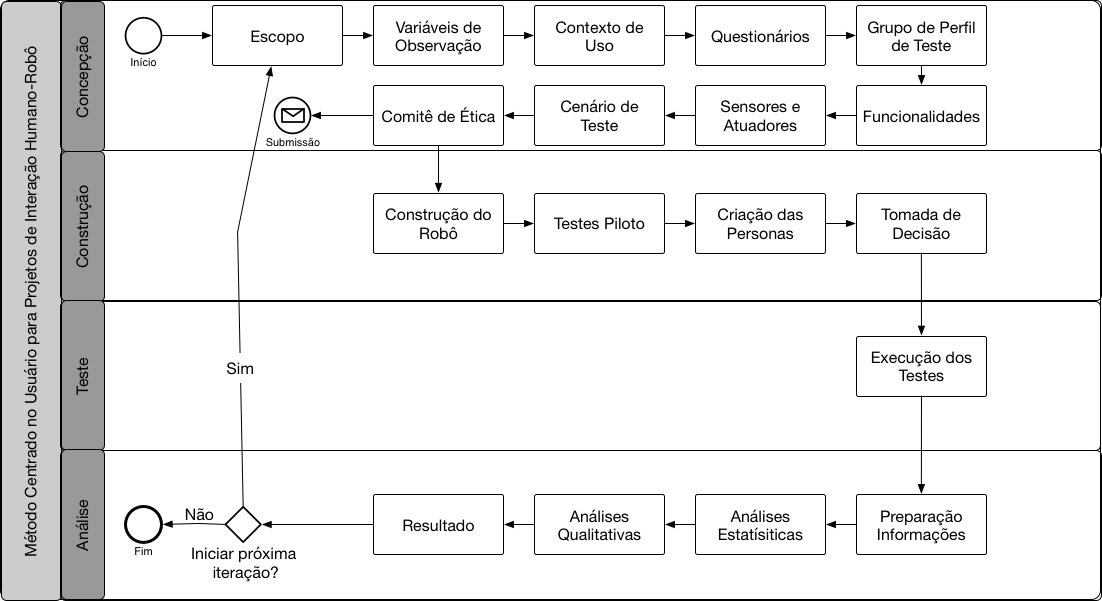
\includegraphics[width=\textwidth]{pool.png}
		\smallcaption{Fonte: o autor.}
		\label{fig:pool}
	\end{minipage}
\end{figure}


Uma explicação detalhada sobre cada etapa contida nas 4 fases do método são apresentadas ao longo do restante deste capítulo.

\section{CONCEPÇÃO DO PROJETO DE INTERAÇÃO HUMANO-ROBÔ}
\label{sec:concepcao}
Essa seção apresentada os detalhes que devem ser contemplados na fase de concepção do projeto de interação humano-robô, utilizando robôs autônomos. Esse é uma etapa importante para a metodologia proposta, pois auxilia na construção de um robô centrado no usuário e capaz de realizar tarefas em um mesmo ambiente com o ser humano. A figura~\ref{fig:concepcao} apresenta de maneira macro a sequência das fases a serem realizadas ao longo da fase de concepção.

\begin{figure}[ht!]
    \centering
    \begin{minipage}{\textwidth}
        \caption{Visão geral da sequência de passos da fase de concepção.}
        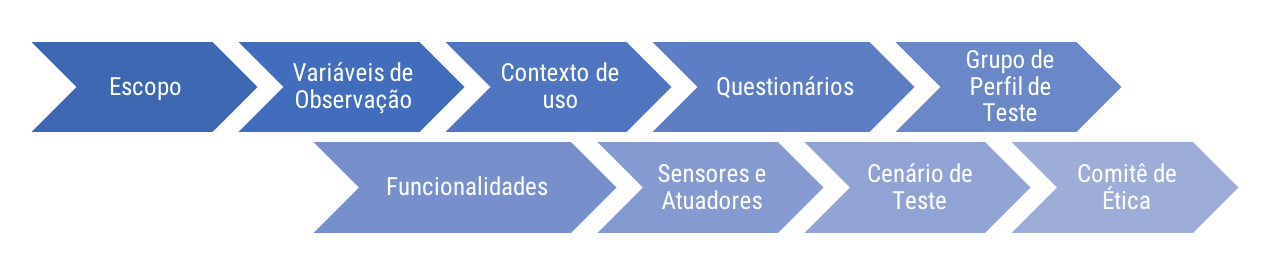
\includegraphics[width=\textwidth]{concepcao.png}
        \smallcaption{Fonte: o autor.}
        \label{fig:concepcao}
    \end{minipage}
\end{figure}

Na sequência é apresentado em detalhes cada um dos passos necessários para conseguir realizar a fase de concepção do projeto de interação humano-robô.

\subsection{Escopo do Projeto de Interação Humano-Robô}
\label{sec:escopo}
A definição do escopo do projeto é o passo mais importante da fase de concepção. Esse passo é uma entrada constante para todos os passos do projeto. O escopo é responsável por definir os limites do projeto e também de cada um dos passos e fases que compõem o projeto. O escopo deve ser criado como uma descrição detalhada do projeto. Essa descrição deve conter informações sobre qual o trabalho que será executado para atender o produto ou serviço desejado. 

É importante que estejam definidos de uma maneira macro as funcionalidades e funções específicas do projeto. Após as definições realizadas para o projeto, é fundamental que esse escopo seja validado para identificar se os limites estabelecidos são suficientes para avaliar o serviço ou produto desejado. Nessa tese o produto desejado é um projeto de interação entre seres humanos e robôs autônomos dentro de um ambiente doméstico.

\subsection{Variáveis de Observação}
\label{sec:variaveis}
As variáveis de observação são importantes para que as informações sejam analisadas dentro do escopo do projeto. Elas auxiliaram a definir quais são os sensores e atuadores necessários para a construção do robô. Essas variáveis devem ser separadas em classes de maneira que seja possível referencia-las como um grupo durante o projeto. As classes definidas nessa tese são etnográficas, comportamentais, do robô e ações na interação, todas discutidas nas seções a seguir. A investigação tem o objetivo de melhorar a interação humano-robô sempre com o foco nas necessidades do ser humano, que é o usuário do sistema. Cada classe de variáveis adotada possuí um conjunto de características e especificidades única para obtenção e análise das informações. Identificar as variáveis é importante, por que auxiliará na definição da maneira de captura de cada uma delas. Por exemplo, a variável nome do usuário, pode ser obtida através da interação por voz com o usuário ou através de questionário prévio aplicado antes da interação e repassado ao robô para interação mais pessoal. O meio de obtenção dependerá do momento e objetivo do projeto.

A escolha do conjunto de variáveis é realizada com base em revisão bibliográfica da literatura da área de interação humano-robô e interação humano-computador. Além disso, conhecimento prévio do especialista também deve ser utilizado para selecionar as variáveis de observação a serem utilizadas no projeto. O objetivo de identificar as variáveis é representar melhor as informações necessárias para análise do problema. Ao longo do capítulo~\ref{cap:ihr}, algumas variáveis para projeto de interação de robôs autônomos foram identificadas. Na literatura, o uso da teoria de proximidade demonstra possibilidades de extração de fatores comportamentais que utilizam como base a distância social, neste caso entre pessoas e o robô. Esses fatores não referem-se apenas sobre a posição física entre dois agentes. Questões de comportamento de interação também são contemplados pela teoria de proximidade. Por exemplo, a orientação dos ombros e tronco em relação a posição do robô (linguagem corporal)~\cite{mead:2016}. A fixação e frequência de olhares pode determinar o início e o fim de uma interação. O olhar também auxilia a determinar quem são os principais indivíduos na interação~\cite{mumm:2011, srinivasan:2012}. O emprego de reconhecimento de expressões faciais para auxiliar na análise do quanto o cenário com o robô é confortável para o indivíduo, ou seja, o quanto ele aprecia e mantém a interação. Existir uma avaliação em tempo real das reações deste indivíduo durante todo o processo de interação, auxilia na compreensão da experiência do usuário~\cite{amaral:2014}. Outra técnica para análise de conforto na interação é a avaliação da emoção através da voz da pessoa, ou através do uso de equipamento de eletroencefalografia~(EEG), porém este último é um método mais invasivo já que exige a adição de um equipamento na pessoa que interage com o robô~\cite{bos:2006, lee:2014}.

Para que essas variáveis sejam capturadas e analisadas de maneira automatizada, é possível empregar diversos sensores para auxiliar na leitura e quantificação delas. Sensores de captura de marcações de movimento, como Microsoft\textregistered\ Kinect\textregistered\ ou o ASUS\textregistered\ Xtion\textregistered, são utilizados para quantificar os valores comportamentais obtidos através das variáveis, que envolvem distância entre agentes e orientação de corpos. Para realizar o reconhecimento de expressões faciais utiliza-se uma câmera de vídeo. Pode-se assim executar a leitura da face da pessoa em tempo de interação. As variáveis referentes a questão da fixação dos olhares dos agentes para identificar o início e o fim da interação, podem ser obtidas através de ambos sensores, sendo possível determinar a orientação da cabeça e torso do indivíduo, além de também a direção do olhar da pessoa para o robô. A voz do indivíduo capturada pelo robô permite a análise da emoção na interação. Ela é obtida através de um microfone direcional ou um arranjo de microfones, que amplifica a capacidade de percepção do robô em relação ao ambiente e a pessoa que interage com ele.

As variáveis aplicadas ao comportamento 	possui dependência do cenário de interação. Entretanto, as informações obtidas com as variáveis etnográficas como idade, experiência computacional, gênero, local de nascimento, etnia, entre outras, são independentes do cenário. Existem alguns algoritmos na área de visão computacional que são capazes de identificar algumas variáveis etnográficas de maneira automática \cite{yang:2007, shan:2012, ylioinas:2012, samadi:2013, amaral:2014}. Essa técnica auxilia na construção de mecanismos de tomada de decisão de maneira automática, deixando a interação com o robô mais autônoma e inteligente. Porém, as informações que não podem ser obtidas de maneira automática, então alguns métodos como questionários e entrevistas são necessários para melhor compreensão do perfil do usuário e identificar sua experiência durante a interação.

Nesta tese são apresentados quatro conjuntos de variáveis consideradas como base para projetos de interação humano-robô. Eles são classificados entre: etnográficas, comportamentais, do robô e de ações de interação. As variáveis etnográficas são apresentadas na seção~\ref{sec:etnograficas}. Na sequência as variáveis comportamentais na seção~\ref{sec:reacoes}. Depois, as variáveis do robô são apresentadas na seção~\ref{sec:variaveisrobo}. E por fim, as variáveis de ações na interação apresentadas na seção~\ref{sec:acoes}.

\subsubsection{Variáveis Etnográficas}
\label{sec:etnograficas}
As variáveis etnográficas têm o objetivo de coletar informações sobre etnia, cultura, costumes e outros fatores antropológicos~\cite{borges:2005}. Além dessas informações, elas auxiliam na identificação de dados sobre idade, gênero, experiência social e tecnológica do indivíduo. Todas as informações representadas nos dados etnográficos são relevantes para verificar a adesão do usuário sobre novas tecnologias, em qual cultura ele está inserido, e outras informações que podem determinar o nível de interação que o usuário aceita com a tecnologia, neste caso o robô. Essas informações podem ser capturadas através de questionários e entrevistas. Caso seja uma necessidade do projeto, o robô pode coletar as informações sobre a etnografia da pessoa através de entrevista verbal. Essas informações podem servir para o especialista identificar preferências do usuário importantes na construção do robô ou até para uma interação mais personalizada do robô. A lista apresentada a seguir define um conjunto mínimo de variáveis etnográficas e uma breve explicação sobre o significado de cada uma:

\begin{enumerate}
    \item \textbf{Idade}: informa a idade do indivíduo.
    \item \textbf{Gênero}: informa o sexo biológico do indivíduo.
    \item \textbf{Local de Nascimento}: informa qual o local de nascimento do indivíduo. Essa variável auxiliará a determinar a base cultural do indivíduo.
    \item \textbf{Etnia}: informa a origem da família do indivíduo. Outra variável que auxilia na determinação da base cultural do indivíduo.
    \item \textbf{Quantidade de \emph{Gadgets}}: informa a quantidade de \emph{gadgets} que o indivíduo possui, ajudando a identificar qual a experiência e o contato dele com a tecnologia.
    \item \textbf{Contato prévio com Robôs}: informa apenas se o indivíduo já possuiu algum contato com robôs. Auxiliará a determinar o contato com a tecnologia, principalmente com robôs que poderá influenciar no seu comportamento durante a interação.
    \item \textbf{Tipos de Robôs}: informa quais são os tipos de robôs que o indivíduo teve contato. Os tipos poderão ser robôs \emph{Pet}, Humanoides, Androides, Móveis, entre outros. Essa variável é um complemento da variável ``Contato prévio com Robôs''.
    \item \textbf{Quantidade de cidades visitadas}: informa a quantidade de cidades que o indivíduo já visitou além da sua cidade natal. É importante para identificar o contato com outros tipos de cultura. Isso poderá influenciar no comportamento definido por sua cultura.
    \item \textbf{Quantidade de cidades que morou}: informa a quantidade de cidades que o indivíduo já morou além da sua cidade natal. É importante para identificar a vivência com outros tipos de cultura. Isso poderá influenciar no comportamento definido por sua cultura.
    \item \textbf{Quantidade de países visitadas}: informa a quantidade de países que o indivíduo já visitou além da sua cidade natal. É importante para identificar o contato com outros tipos de cultura. Isso poderá influenciar no comportamento definido por sua cultura.
    \item \textbf{Quantidade de países que morou}: informa a quantidade de países que o indivíduo já morou além da sua cidade natal. É importante para identificar a vivência com outros tipos de cultura. Isso poderá influenciar no comportamento definido por sua cultura.
\end{enumerate}

Em diversos trabalhos do capítulo~\ref{cap:ihr}, onde a questão cultural do indivíduo é abordada, é discutido sobre influência que a cultura provê no comportamento do indivíduo. A cultura é tratada como o local de nascimento da pessoa~\cite{eresha:2013}. Entretanto, a questão cultural na vida de uma pessoa é mais abrangente pois, pode ser relacionada com a experiência adquirida ao longo de sua vivência social, como por exemplo, países e cidades que o indivíduo visitou e viveu, o meio ao qual ele está inserido, sua profissão, entre outras informações. Dessa forma, o conjunto de variáveis apresentado na lista acima auxilia a mapear de forma macro a experiência social e de vida do indivíduo. O uso das informações etnográficas tem o objetivo de investigar até que ponto elas podem influenciar na experiência do usuário durante a interação com o robô.

\subsubsection{Variáveis Comportamentais}
\label{sec:reacoes}
Variáveis comportamentais tem como principal objetivo identificar os estímulos do usuário dentro do cenário que contém uma determinada tarefa. As variáveis comportamentais são coletadas a partir de informações encontradas em expressões corporais, faciais, no uso do sistema e na declaração explícita da pessoa ou do robô. O uso de variáveis comportamentais possibilita uma análise baseada em teorias de linguagem corporal e de microexpressões~\cite{lambert:2008}. No trabalho apresentado por \textcite{lambert:2008} são discutidos os significados de 101 expressões corporais identificadas ao longo de sua pesquisa. O conjunto de variáveis comportamentais apresentados nessa seção podem ser utilizados não apenas para extrair o perfil comportamental do indivíduo, mas também para avaliar a ação realizada pelo robô ao interagir com o usuário. Dependendo do \emph{hardware} utilizado no robô, essas variáveis também possibilitam que o robô realize a imitação dos comportamentos durante a interação como um aprendizado por observação ou trabalho de espelhamento do comportamento. A lista apresentada a seguir define as variáveis comportamentais obtidas através da literatura estudada nessa tese e uma breve explicação sobre o objetivo de cada uma das variáveis:

\begin{enumerate}
    \item \textbf{Expressões Faciais}: é possível identificar se a reação do indivíduo foi positiva ou negativa, a partir de uma ação do robô. Existem seis expressões bases que combinadas formam diversas outras~\cite{bihan:2014}. É sugerido por este trabalho considerar apenas as seis expressões bases (raiva, nojo, medo, feliz, triste e surpreso~\cite{kaitai:2011}), classificadas em dois grupos: expressões faciais positivas e expressões faciais negativas. O intuito dessa variável é realizar a avaliação da ação do robô com base nas expressões faciais do indivíduo. Caso identifique a necessidade dentro do cenário de atuação, o detalhe desta variável pode tornar-se interessante. As percepções são feitas pelo especialista durante o experimento ou implementado no robô com o uso de bibliotecas de visão computacional, algoritmos de classificação e o uso de uma câmera para obter a imagem.
    \item \textbf{Tempo de Aproximação}: identificar o tempo que o robô levou para se aproximar do indivíduo sem gerar situações de desconforto, como por exemplo, afastar-se do robô, expressar alguma face negativa, ou posições do corpo que repassem uma imagem negativa, como braços cruzados e tronco inclinado levemente para trás.
    \item \textbf{Orientação do Olhar ao Robô}: identificar a orientação do olhar que indivíduo mantém ao robô, sendo possível saber se a interação está continua ou não. Isso pode influenciar se o robô está interagindo de maneira confortável ao indivíduo ou se esse está incomodado com a presença do robô.
    \item \textbf{Tempo do Olhar}: é possível mensurar o interesse do indivíduo durante a interação através do tempo que ele permanece com o olhar fixo no robô. Quanto maior o tempo do olhar, maior o interesse na interação do indivíduo.
    \item \textbf{Orientação dos ombros}: Auxilia a mensurar o interesse do indivíduo durante a interação. Ao analisar se os ombros possuem a mesma orientação que a cabeça e também uma orientação em direção ao indivíduo que interage com o robô é possível inferir seu objetivo e interesse pela interação. Além disso, é possível determinar através do alinhamento do quadril com o ombro do indivíduo o ângulo de inclinação de seu torso. A inclinação do torso auxilia a identificar quanto o indivíduo está interessado na interação, para isso basta verificar se ele está inclinado em direção ao robô para determinar um interesse positivo~\cite{lambert:2008}.
    \item \textbf{Orientação do quadril}: Auxilia a mensurar o interesse do indivíduo durante a interação. A orientação do quadril em direção ao robô ou na direção oposta auxilia a determinar o grau de interesse do indivíduo na interação. Quando mais alinhado à direção do robô, maior o interesse do indivíduo na interação~\cite{lambert:2008}. Essa variável pode ser trabalhada em conjunto a orientação dos ombros.
    \item \textbf{Estilo da Voz}: é importante, pois pode determinar a reação que o indivíduo terá após a interação via áudio com o robô. Além disso, é possível determinar se o indivíduo está confortável ou não durante a interação, analisando o tom de sua voz ao responder o robô. A análise de emoção através de áudio é uma tarefa complexa e deve ser considerada para robôs de serviço que irão atuar em ambientes domésticos.
    \item \textbf{Conforto}: determina se o indivíduo está disposto a continuar a interação ou se algo o incomoda, fazendo com que desista de interagir com o outro agente. Essa é uma informação que pode ser obtida através das demais apresentadas acima ou de forma declarada diretamente pelo usuário por voz.
    \item \textbf{Medo}: determina se o indivíduo sente-se seguro durante a interação com o robô. Pode impactar diretamente a experiência de interação do usuário. Essa é uma informação que pode ser obtida através das demais apresentadas acima ou declarada diretamente pelo usuário por voz.
\end{enumerate}

As variáveis apresentadas acima podem auxiliar na descoberta do interesse em relação a interação, além de sua apreciação. Algumas delas, como as que envolve o olhar, podem necessitar de equipamentos mais específicos para obter uma melhor acurácia na captura. Outras variáveis necessitam de técnicas e estudos direcionados para trazer a interação à um nível mais natural, como o caso da voz. Dessa forma, escolher quais variáveis trabalhar tem influência não só sobre o estudo realizado, como também nos equipamentos embarcados no robô. Tais equipamentos, podem influenciar em sua aparência e consequentemente na experiência do usuário.

\subsubsection{Variáveis do Robô}
\label{sec:variaveisrobo}
Além das variáveis referentes a etnografia e comportamento, deve-se considerar também as informações sobre o robô uma vez que sua aparência pode influenciar na reação e expectativa das pessoas durante a interação~\cite{hegel:2009}. Variáveis do robô podem auxiliar a identificar quais são os principais fatores de sua aparência que tornam a interação humano-robô uma boa experiência ao usuário. Também pode-se investigar a naturalidade permitida pelo \textit{hardware} utilizado em sua construção. Um conjunto de variáveis é apresentado com o objetivo de caracterizar fatores do robô, referente a sua aparência, que influenciam na interação social. Esse conjunto de variáveis é apresentado a seguir:

\begin{enumerate}
    \item \textbf{Altura}: A altura do robô para identificar a influência da diferença entre alturas de robôs e humanos.
    \item \textbf{Volume}: O volume ocupado pelo robô pode influenciar no conforto da interação, uma vez que quando o robô atingir uma zona social mais próxima do indivíduo pode causar uma sensação claustrofóbica a ele.
    \item \textbf{Tipo do Robô}: Segundo \textcite{choi:2014}, robôs possuem dois tipos: Autônomos e Tele-operados. Essa variável define o quanto de intervenção humana é necessário para que o robô possa executar a tarefa objetivo.
    \item \textbf{Classificação do Robô}: Segundo \textcite{dobra:2014} classificar um robô é uma tarefa muito complexa e pode envolver diversas variáveis. Dessa forma, para essa tese será considerado uma classificação mais simples. O robô deve ser classificado como: fixo, móvel com rodas, móvel bípede, móvel quadrupede, móvel com manipuladores. Outras classificações podem ser inseridas conforme a necessidade e inclusão de novos robôs.
    \item \textbf{Aparência Física}: Essa variável descreve se o robô possui uma aparência amigável ou agressiva. Essa variável depende da preferência do usuário, mas a parte do formato físico do robô pode influenciar na percepção desta variável.
    \item \textbf{Nível de Ruído}: Determina qual o nível de ruído que os atuadores e sensores do robô podem gerar de tal forma, que possa influenciar na interação humano-robô. Como exemplo, pode-se citar o Big Dog~\footnote{http://www.bostondynamics.com/robot\_bigdog.html}, da Darpa Robotics, que é movido através de um motor diesel e seus atuadores pneumáticos e hidráulicos apresentam um alto grau de ruído.
\end{enumerate}

\subsubsection{Variáveis de Ações na Interação}
\label{sec:acoes}
Existem variáveis que determinam as possíveis ações que o robô e o ser humano podem executar, uma vez que o robô é o elemento ativo durante o experimento. Essas ações podem gerar comportamentos diferentes de acordo com o contexto ao qual o cenário está inserido. No caso do robô, as possíveis ações são determinadas a partir do \emph{hardware} disponível para o projeto. Fatores como tipo de manipulador, sonorização, saída de vídeo, entre outros, determinam quais são as ações que habilitem o robô executar. As variáveis que compõem as informações das possíveis ações que o robô pode executar são:

\begin{enumerate}
    \item \textbf{Aproximação}: Forma de aproximação do robô ao indivíduo. Pode ser classificada entre rápida, devagar, brusca ou suave.
    \item \textbf{Movimentação do Manipulador}: Caso exista um manipulador deve descrever como é feita a movimentação do manipulador em direção ao usuário. A classificação pode ser feita entre brusca e suave; ou em relação a sua amplitude, como longo e curto.
    \item \textbf{Estilo de Voz}: Ao emitir algum tipo de som o robô deverá manter um estilo de voz para que seja possível simbolizar qual o tipo de mensagem ele deseja falar. A classificação será feita de maneira simplificada, considerando apenas se é um estilo educado ou agressivo.
    \item \textbf{Volume de Voz}: Ao emitir um som, o robô deve saber qual o volume adequada considerando a interação, ambiente e distância do segundo agente. Uma classificação simples pode ser utilizada, como por exemplo, alto e baixo.
    \item \textbf{Expressão Facial}: Ao iniciar o contato visual com o indivíduo, pode ocorrer diversas expressões do robô na tentativa de manter o conforto do indivíduo durante o processo de interação. Simplificando as expressões são consideradas apenas dois tipos de expressões realizadas pelo robô: amistoso e não-amistoso. As expressões faciais do robô poderão ser executadas através de um \emph{tablet} acoplado nele.
\end{enumerate}

A partir das variáveis identificadas, deve-se realizar a definição do contexto de uso para definir quais e como são utilizadas cada uma das variáveis no projeto de interação humano-robô proposto. Elas devem ser necessárias para atender os objetivos de interação apresentados a partir do contexto de uso. O contexto de uso é detalhado na seção~\ref{sec:contextouso}

\subsection{Contexto de Uso}
\label{sec:contextouso}
O contexto de uso possui influência direta na interação das pessoas com os sistemas interativos. Dependendo do contexto, cada pessoa irá agir de acordo com a influência de sua cultura, sociedade e outras questões externas. Uma pessoa executa as tarefas de maneira única com modos desenvolvidos ao longo de sua vida, baseando-se na educação obtida através de sua família. Essa base exerce força sobre os conhecimentos prévios, concepções e linguagens utilizadas durante o processo de interação. O contexto de uso utilizado para análise dos usuários no processo de interação é diferente do contexto aplicado ao cenário de desenvolvimento em geral. Para desenvolvedores o contexto é apenas os limites de aplicação do projeto. O contexto de uso apresentado nessa seção, tem relação com o ambiente de aplicação do produto e o local onde o usuário consumirá esse sistema.

É importante dar ao contexto de uso um ambiente natural ao usuário, um local onde ele faria o uso, de maneira real, do sistema. Isso influência diretamente o tipo de análise que deve ser realizado. Além de auxiliar diretamente nas diretrizes de construção e consequentemente na análise dos resultados obtidos durante os testes. A definição do contexto de uso é baseada em um texto descritivo que delimita todo o cenário da aplicação e como foi planejado o experimento. Esse cenário descreve quem é o usuário, quais os pontos de interação com o sistema, como será o comportamento do usuário e do robô. O contexto descrito delimita todo o escopo do teste. Ele assegura que as observações tenham o objetivo de garantir a qualidade do uso dentro do ambiente investigado. 

\subsection{Questionários}
\label{sec:questionarios}
Questionários são formulários que podem ser impressos ou construídos em sistemas que utilizem a internet. Neles são realizados uma coleta de informações sobre o que o usuário, participante do teste, sente ou pensa em relação ao produto em análise. Esse formulário é composto por perguntas que podem ter características que a deixem fechadas ou abertas. No caso de questionários a recomendação é forte para perguntas fechadas por proporcionarem uma análise mais fácil e também serem mais rápidas para responder.

Esse meio de coleta de informações tem uma vantagem perante a outros métodos como percurso cognitivo, entrevistas e grupos focais. Nele a distribuição pode ser realizada a pessoas que estejam geograficamente dispersas, fazendo com que elas possam responder a qualquer horário e em qualquer lugar. No caso dos projetos de interação humano-robô, essa distribuição geográfica não é interessante, pois existe a necessidade de realizar o teste de interação com o robô, posteriormente, a fim de validar o experimento social com o robô após um teste presencial.

Para preencher o questionário, cada pessoa desprende de um certo tempo para responder as perguntas contidas nele. Esse tempo deve ser respeitado e ainda é importante que a pessoa encontre-se em um ambiente confortável para que ele se sinta a vontade ao respondê-lo. No caso dos testes realizados com interação humano-robô, recomenda-se que utilize esse tempo de resposta para preparar o início do teste com o robô. Essa preparação consiste em liberá-lo da energia elétrica, acertar a captura de dados dos sensores e também preparar o mecanismo de controle e tomada de decisão com o robô. Toda essa preparação deve ser realizada em um ambiente separado ao do preenchimento do questionário para não distrair o participante do teste.

A comunicação com o participante durante esse período é restrita, devendo ser mínima, de preferência nula. É importante que isso se mantenha, para que evite tendências nas respostas influências pela opinião e conversa do especialista. Dessa maneira, cada pergunta deve ser realizada de forma a ter um fácil entendimento. Deve-se evitar ambiguidades e mal-entendimentos. Uma boa prática para essa situação é envolver uma pessoa que não participou da criação do questionário e solicitar que ela leia as perguntas em voz alta, dizendo o que entendeu sobre cada uma delas. Assim, é possível validar a falta de ambiguidades e mal-entendimentos.

Ao estruturar um questionário é importante coletar informações demográficas básicas, como gênero e idade, além de informações sobre a experiência da vida do usuário, a tecnológica e também a experiência prévia sobre o produto que irá interagir, no caso o robô. Outras informações importantes são as declaradas sobre a experiência com a interação realizada durante o teste com o robô. No caso da interação entre o usuário e o robô, recomenda-se separar as informações mencionadas entre dois questionários, um de pré e outro de pós teste de interação. No questionário pré teste inclui-se as perguntas referentes as informações demográficas básicas e experiências prévias de vida, tecnológica e com o produto. É importante também existir uma informação que possa vincular os registros de respostas entre o pré e o pós questionário.

No questionário pós teste encontram-se as perguntas referentes a experiência de interação com o produto, no caso o robô, contendo informações essenciais à análise do produto. O tipo de resposta escolhida para cada pergunta irá influenciar no tipo de análise realizada mais a frente. Respostas fechadas que utilizem escalas de Likert, múltiplas escolhas ou por faixa de valores, auxiliam em análises quantitativas. Já as respostas abertas, de texto corrido, permitem uma análise qualitativa, pois é necessária sua leitura por um especialista para que ele consiga interpretar as informações que são relevantes ao processo de análise. Esse ponto será abordado mais na seção~\ref{sec:analise} apresentada mais a frente neste capítulo. 

\subsection{Seleção do Grupo de Perfis de Teste}
\label{sec:selecaoperfis}
Nessa etapa é analisado as características mais importantes dos usuários que irão compor o grupo de teste. É uma tarefa que deve ser realizada com muita atenção, pois aqui é selecionado o público alvo do projeto de interação humano-robô. Aqui são estimados os intervalos que irão compor a idade dos usuários. Quais são as principais características e conhecimentos sobre a tecnologia aplicada durante o teste. Todas essas informações são importantes para determinar as diretrizes que o projeto irá seguir e como será validado e publicado as informações. Essa seleção faz parte da estratégia que o projeto irá seguir em sua construção e qual o foco que será dado a criação da aparência do robô.

O principal intuito da seleção de grupo de perfis de teste é estipular uma amostra mais próxima da realidade ao seu perfil real de consumidores do produto. Para a seleção deve-se pensar em quais atividades esses usuários irão realizar com o robô e como eles podem se envolver nos testes. Para cada um desses usuários deverá ser apresentado um termo de consentimento e esclarecido quais são os objetivos do teste. Informar se existe ou não o risco de se machucar durante o teste, pois nesse caso o robô pode acabar realizando alguma ação não prevista devido sua autonomia e até mesmo ruídos na leitura do sensor. 

Questões de bonificações deverão ser pensadas nessa etapa, pois isso pode trazer outros fatores ao teste, como interesse apenas na remuneração. Recomenda-se que os testes sejam executados de maneira voluntária evitando qualquer tipo de questionamento ao real intuito do resultado. Esse é um fator que impacta diretamente na seleção do perfil, pois deverá ser previsto um perfil que esteja mais voltado a ajuda real dos testes realizados. A seleção é importante, pois é um dos passos fundamentais para a construção de um projeto apoiado pelo comitê de ética, que será discutido em mais detalhes na seção~\ref{sec:comiteetica}.

\subsection{Funcionalidades}
\label{sec:funcionalidades}
Realizar uma boa especificação de projeto de \textit{software} é importante para o seu sucesso. Projetos sem especificações são difíceis de serem reproduzidos, uma vez que os robôs utilizados são bem específicos. Além de serem específicos, os robôs utilizados são construídos, nos laboratórios das universidades e centros de pesquisas, em parte das pesquisas. Outras pesquisas utilizam robôs como: Softbank NAO~\footnote{https://www.ald.softbankrobotics.com/en/robots/nao} e PR2~\footnote{http://www.willowgarage.com/pages/pr2/overview}. Eles são produzidos por empresas especializadas fazendo com que o projeto fique restrito a capacidade determinada pela fábrica.

Em engenharia de \emph{software} são estudados vários métodos que auxiliam na especificação do projeto. Nesses métodos são encontrados a contemplação de alguns princípios que garantem a reprodução, manutenção e evolução do projeto ao longo tempo. Os princípios de engenharia de \emph{software} não são vistos como regras, mas como boas práticas para o desenvolvimento do projeto~\cite{wazlawick:2013}. As boas práticas aplicadas em sistemas computacionais, também podem ser aplicadas no desenvolvimento de projetos de robôs. Em seu trabalho \textcite{wazlawick:2013} apresenta algumas boas práticas que a engenharia de \emph{software} provê aos projetos. A lista a seguir, descreve as boas práticas que contribuem para a evolução e formalização do projeto dessa tese:

\begin{itemize}
    \item \textbf{Decomposição}: é a criação de um \emph{software} ou produto a partir de um conjunto funcional de alto nível, os requisitos do projeto, onde esses são divididos em partes mais simples até chegar a um produto atômico, ou seja, partes de códigos. No robô, pode-se incluir também como os sensores e atuadores do projeto.
    \item \textbf{Padronização}: são importantes pois, através dos padrões conhecimentos adquiridos em projetos passados podem ser aplicados nos atuais evitando assim, que erros similares sejam cometidos.
    \item \textbf{Flexibilização}: auxilia na acomodação das mudanças de requisitos do projeto, No caso de robótica, nos cenários de atuação, diferentes contextos de uso, novos sensores e plataformas, entre outros.
    \item \textbf{Desenvolvimento Iterativo}: a cada momento novas necessidades são criadas e a partir da criação deve ser inserida no projeto. Nas metodologias iterativas, cada ciclo de desenvolvimento é independente e deve entregar um produto operacional. Ao tratar de um projeto de interação humano-robô, pode-se dizer que o processo iterativo é longo e não necessariamente finito. Isso ocorre devido as novas necessidades dentre os diversos contextos de uso como hospitais, casas, hotéis, museus, resgate, shoppings, entre outros.
    \item \textbf{Arquiteturas baseadas em Componentes}: auxilia a lidar com complexidade do projeto e também o reuso e expansão. Cada sensor novo inserido no robô deve ser inserido junto a um novo módulo que captura as informações, consome os dados e entrega as informações para os componentes de tomada de decisão do robô, por exemplo.
\end{itemize}

Para garantir que as boas práticas sejam aplicadas no projeto, é necessário o uso de algumas ferramentas utilizadas dentro processo de criação de \emph{software}, aqui nessa tese utilizada na criação do projeto de interação humano-robô. O primeiro passo é definir as funcionalidades do sistema, que representam as ações que o robô pode executar. Para criação das funcionalidades do robô utiliza-se as informações obtidas através do contexto de uso (vide seção~\ref{sec:contextouso}), das variáveis de observação selecionadas (vide seção~\ref{sec:variaveis}) e dos perfis de teste (vide seção~\ref{sec:selecaoperfis}). As variáveis de observação são selecionadas e em conjunto com o contexto de uso, deve-se iniciar um processo de \textit{brainstroming} para identificar os requisitos funcionais que estão contidos nas funcionalidades. A determinação do escopo é muito importante para identificar quais são as tarefas que o robô realizará durante a interação social com o ser humano. 

Nesse momento, é uma boa prática revisitar a definição do escopo do projeto para realizar uma análise mais profunda sobre as funcionalidades que tem potencial para serem contemplas. Em algum momento do projeto, pode ocorrer algum problema externo, como a quebra de um sensor fundamental para aquela funcionalidade, e não conseguir cumprir com o planejado. Por isso, é importante determinar as funcionalidades potenciais, a fim de identificar o melhor caso de resultado do projeto. Cada funcionalidade deve ser capaz de atender um requisito do projeto, e deve ser planejada no momento da construção do projeto. Depois é revisado os sensores e atuadores que contribuem com o escopo para cada funcionalidade, vide a seção~\ref{sec:sensoresatuadores}.

\subsection{Sensores e Atuadores}
\label{sec:sensoresatuadores} 
Com as funcionalidades especificadas, o próximo passo é definir quais são os sensores e atuadores as atendem. Cada sensor deve ser pensado de maneira que ele possa coletar as informações necessárias para análise e tomada de decisão do robô perante a funcionalidade que ele deve possuir. Esse conjunto irá determinar a posição que o sensor deve ser adicionado no robô. Além dos sensores, é importante que os atuadores sejam adicionados para contribuir com a execução das tarefas de interação. Os atuadores fazem o robô se locomover, interagir e manipular com o cenário ou usuário. Eles também podem auxiliar no posicionamento adequado dos sensores. A combinação dos sensores com os atuadores deixa a tarefa mais dinâmica e flexível. Eles são importantes também possam tornar as interações cada vez mais naturais. Por isso, é importante que cada um desses componentes deve ser escolhido de acordo com as funcionalidades.

\subsection{Cenário de Teste}
\label{sec:cenarioteste}
O cenário de teste é responsável por descrever as situações de uso existentes dentro de uma determinada tarefa. Como essa tarefa está inserida dentro do contexto de uso, a criação desse cenário deve ser realizada quase como uma transcrição dele. Sua descrição deve ser realizada mais detalhada contendo algumas possibilidades dentre as situações. É importante que a sua descrição gere uma motivação para que o teste ocorra ao mesmo tempo que sua avaliação de sucesso seja feita de maneira simples. Um ponto importante ao definir-se cenários de teste é a possibilidade de testar diversas funcionalidades em um único cenário. 

Caso exista mais do que um cenário isso auxilia na construção de um sistema de teste mais robusto, que irá validar as funcionalidades do sistema em diversos níveis. Além do descritivo, é importante, no cenário de teste para projeto de interação humano-robô, pensar na posição do ser humano dentro do ambiente de teste. Este, por sinal, também deve ser descrito de maneira a atender todas as possibilidades contempladas nos cenários de teste. Agora, com todos esses passos de planejamento, concepção do projeto, pode-se realizar a confecção do projeto para envio ao comitê de ética, tratado na seção~\ref{sec:comiteetica}. A aprovação do comitê de ética é importante, pois todo teste envolve o ser humano e pode ocorrer algum incidente. Essa aprovação auxilia na validação de um produto que não seja prejudicial ao ser humano.

\subsection{Projeto ao Comitê de Ética}
\label{sec:comiteetica}
Todos os passos anteriores, contém informações importantes para a construção do projeto ao comitê de ética brasileiro. Na criação do projeto é importante identificar diversos pontos que devam mitigar qualquer problema ao usuário, participante do teste. Um modelo para a criação do projeto ao comitê de ética brasileiro, recomendado por essa tese, mantém a seguinte estrutura:

\begin{itemize}
	\item \textbf{Introdução}: apresentação das metodologias, motivações e justificativas sobre o projeto;
	\item \textbf{Objetivos}: guiam a construção do seu projeto e ajudam a avaliar o sucesso da tarefa.
	\item \textbf{Hipóteses}: descreve o que deve ser validado após a execução dos testes.
	\item \textbf{Benefícios}: descreve quais são os ganhos ao ter o produto no mercado, inclusive os pontos positivos para a sociedade em geral.
	\item \textbf{Metodologia}: descreve a metodologia utilizada para construção do produto e principalmente para execução dos testes a serem realizados.
	\begin{itemize}
		\item \textbf{Sujeito de Teste}: descrição dos perfis de teste (seção~\ref{sec:selecaoperfis}).
		\item \textbf{Procedimentos Experimentais}: descrição dos cenários de teste (seção~\ref{sec:selecaoperfis}).
		\item \textbf{Dados Experimentais Coletados}: descrever o que será coletado durante os testes.
		\item \textbf{Processamento e Análise dos Dados Coletados}: descreve como será realizado as avaliações dos testes e como serão processadas essas informações.
	\end{itemize}
	\item \textbf{Riscos}: quais são os riscos para o sujeito de teste ao participar do experimento.
	\item \textbf{Desfecho Primário}: qual é a intenção do teste, como um objetivo descrito de maneira mais simples.
	\item \textbf{Cronograma de Execução}: cronograma do planejamento do trabalho.
	\item \textbf{Financiamento}: detalhes sobre custo do projeto, equipamentos e quem é o principal patrocinador. Esse é um item importante para fiscalização financeira, caso exista necessidade no futuro, principalmente perante ao cenário atual do Brasil.
	\item \textbf{Equipe Executora}: quem são os membros da equipe e quais são seus respectivos papéis.
\end{itemize}

O projeto dever ser submetido a avaliação do comitê de ética através da Plataforma Brasil~\footnote{http://plataformabrasil.saude.gov.br/login.jsf}, que está ligada ao ministério da saúde do Governo Brasileiro. Esse processo demora em torno de 90 dias, portanto deve estar na fase de concepção do projeto. Ao escrevê-lo deve-se pensar na evolução do projeto, para que seja contemplado alguns ciclos da iteração do projeto, pelo menos. Caso não seja feito dessa maneira, durante a fase de análise será necessário a submissão de um novo projeto, para cada ciclo de evolução do projeto.

\section{CONSTRUÇÃO DO PROJETO DE INTERAÇÃO HUMANO-ROBÔ}
\label{sec:construcao}
Essa seção apresentada os detalhes que devem ser contemplados na fase de construção do projeto de interação humano-robô, utilizando robôs autônomos. Esse é uma etapa que contempla definições de arquitetura, projeto mecânico e de \textit{software} para sequência da metodologia proposta. Nessa etapa testes pilotos são executados para auxiliar na definição do perfil do usuário, para análise automática do robô. Toda a metodologia para criação desse perfil é contemplado nessa etapa do projeto. O foco do projeto é sempre realizar uma construção do robô centrado no usuário. A figura~\ref{fig:construcao} apresenta de maneira macro a sequência dos passos contidos dentro da fase de construção.

\begin{figure}[ht!]
    \centering
    \begin{minipage}{\textwidth}
        \caption{Visão geral da sequência de passos da fase de construção.}
        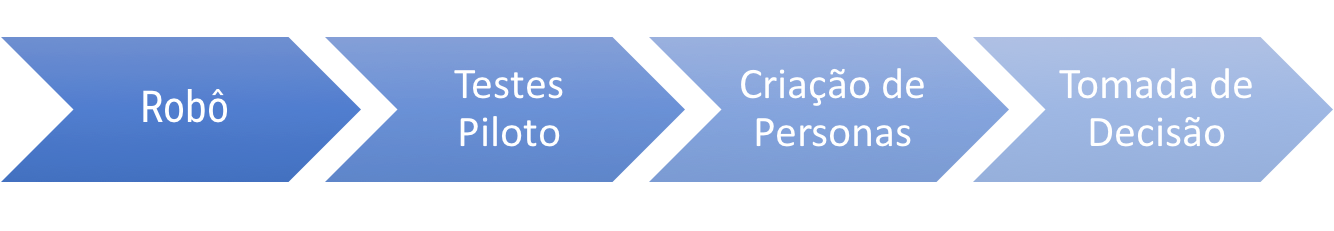
\includegraphics[width=\textwidth]{construcao.png}
        \smallcaption{Fonte: o autor.}
        \label{fig:construcao}
    \end{minipage}
\end{figure}

Na sequência é apresentado em detalhes cada um dos passos necessários para conseguir realizar a fase de construção do projeto de interação humano-robô.

\subsection{Robô}
\label{sec:robo}
Essa etapa é dividida em duas partes que devem ser consideradas no projeto. A primeira parte é o projeto mecânico do robô e o segundo o projeto de \textit{software} dele. Cada particularidade das divisões feitas são discutidas a seguir, nas seções subsequentes.

\subsubsection{Projeto Mecânico}
\label{sec:mecanica}
Com as funcionalidades, sensores e atuadores definidos na fase anterior, é necessário identificar como será a construção física do robô. Será mais vantajoso comprar um produto de prateleira encontrado no mercado, realizar uma modificação nesse produto ou construir um projeto totalmente novo. Aqui é uma etapa que a aparência é importante, mas acima de tudo o projeto deve atender o mínimo de questões de segurança. Recomenda-se realizar protótipos de peças com o uso de impressora 3D. Dependendo da construção e da quantidade de peso que será necessário carregar uma versão final utilizando a impressora 3D pode ser mantida. Caso o material da impressão seja menos resistente, outras opções são possíveis, como fibra de carbono ou alumínio.  A questão sobre o material a utilizar é a relação de peso e autonomia de bateria que isso ocorre. É sempre bom pensar no material mais resistente pelo menor pesos, isso acarretará em uma autonomia de bateria maior. O projeto mecânico deve levar essas informações em consideração, pois caso contrário a autonomia de robô é mínima.

\subsubsection{Projeto de Software}
\label{sec:software}
Nessa etapa que deve ser considerado todas as questões de inteligência e controle do robô. Alinhar as informações dos sensores para que os atuadores contemplem com precisão o trabalho designado a isso. Nessa etapa, além dos algoritmos de controle que devem ser construídos pensando em cada atuador, é importante identificar a arquitetura do \textit{software} utilizado. O ideal é trabalhar com um modelo de arquitetura em camadas. Cada camada deve conter uma única responsabilidade evitando assim trabalho dobrado dentro das questões de \textit{software} do projeto de interação humano-robô.

Junto com a arquitetura é definido também quais são as bibliotecas que serão utilizadas no controle, tomada de decisão e auto teste do robô. O uso de bibliotecas pode auxiliar a direcionar todo o esforço para criação de algoritmos e técnicas que não foram consideradas em seu trabalho, ou seja, as novas técnicas. Também é importante para utilizar quando o algoritmo já implementado nas bibliotecas não atendem por completo suas necessidades. Nesse ponto é preciso reutilizar uma parte do código para desenvolver uma versão personalizada da biblioteca escolhida. Para robô que contemple computadores de pessoais como seu cérebro, utilizar o ROS (\textit{Robot Operating System}) para realizar o desenvolvimento do software. Ele mantém a arquitetura em camadas e pode facilitar o trabalho de \textit{plug 'n play} dos componentes mecânicos e eletrônicos do robô. Além disso, grande parte dos robôs de prateleira do mercado utilizam o ROS como seu sistema principal.

\subsection{Testes Piloto}
\label{sec:testepiloto}
Com o robô construído é importante que seja realizado o teste piloto. Para o teste, toda documentação e artefatos a serem consumidos, devem estar prontos, inclusive a aprovação do projeto no comitê de ética. Em um projeto tradicional, executar apenas um teste piloto, é necessário para que valide os artefatos a serem produzidos e também do cenário de teste. Entretanto, esse não é um projeto tradicional. Nesse momento é importante que ocorram uma bateria de testes pilotos, para levantar informações dos perfis dos usuários alvo do projeto. A partir desses perfis, serão levantadas informações sobre cada característica marcante dos perfis, agrupados os perfis similares e com esses agrupamentos serão produzidos Personas para auxiliar na adaptação do comportamento do robô perante o usuário.

Os testes pilotos devem ser executados com uma diversidade de perfis para que as Personas produzidas consigam contemplar um grande intervalo de perfis no mundo real. Quanto maior a diversidade, maior será a qualidade das Personas produzidas, pois elas possuirão características bem diferentes entre si. Não existe um número para dizer quantos testes são suficientes, alguns estatísticos recomendam um número de 30 testes, porém nesse caso seria necessário um número de 30 perfis de cada tipo para atender essa recomendação. Porém, a recomendação sobre o que não se deve fazer é utilizar menos do que 10 testes, pois com esse número o resultado não é robusto, uma vez que ele corre o risco de ficar tendencioso a um único perfil.

\subsection{Criação das Personas}
\label{sec:criacaopersonas}
O primeiro passo é resgatar as informações dos questionários respondidos e consolidar em uma única base de dados. Essa base pode ser um sistema relacional, não relacional e até mesmo um arquivo do tipo CSV (\textit{Comma-Separated Values}). A recomendação é de uso do arquivo CSV, pois é o mais simples de ser manipulado nesse caso. O uso do arquivo, deve-se contemplar com sendo cada linha um perfil de usuário que realizou o teste.

A partir da base de dados criada com as informações dos questionários, deve-se remover as informações de texto livre, uma vez que o algoritmo não possui um interpretador semântico. Sem o interpretador semântico, não é possível criar um modelo quantitativo para as respostas, onde exista uma significância comparativa.

As informações existentes nos questionários podem ser quantificadas, por exemplo a idade do usuário. A comparação de similaridade entre duas idades pode ocorrer com medidas de distância, por exemplo, a distância euclidiana. Outras medidas também podem ser aplicadas, porém dependerá do tipo de informação e necessidade do projeto~\cite{masiero:2011, masiero:2013}. No caso do agrupamento de perfis desta tese, para informações numéricas, a distância euclidiana é adotada. Ela atende a necessidade do algoritmo e do processo para agrupamento dos perfis.

Variáveis categóricas, ou seja, as variáveis que possuem um valor textual que podem ser separadas em categorias, deve-se realizar um tratamento para quantificá-las. Existem duas opções para quantificar as variáveis categóricas. A primeira opção é inserir um código numérico para cada valor, por exemplo, os valores ``Celular, Computador, Tablet, Autoatendimento, Caixa Físico'' recebem um valor representado por um número inteiro cada ficando ``Celular = 1, Computador = 2, Tablet = 3, Autoatendimento = 4, Caixa Físico = 5'', conforme~\citeonline{masiero:2013}. A segunda opção é transformá-las em variáveis \emph{dummies}~\footnote{http://pandas.pydata.org/}. O método \emph{dummies} transforma cada opção de resposta ou cada categoria em uma nova variável binária onde o valor 1 é para quando a opção for verdadeira e 0 para o oposto.

Realizado os procedimentos para quantificar todas as variáveis, a base de dados já pode ser inserida no algoritmo para o processo de agrupamento. Porém, um outro detalhe nos dados é importante para evitar o problema de tendência no algoritmo. Cada variável possui uma escala diferente. Essa diferença na escala das variáveis pode gerar as tendências no resultado do algoritmo. Assim, é necessário padronizar os valores numéricos existentes na base dentro da mesma escala. Para realizar a padronização dos dados o processo de normalização é executado. A normalização mais comum a ser feita é manter os valores das variáveis entre 0 e 1~\cite{lattin:2011}. A equação~\ref{eq:normalizacao1} apresenta a forma mais simples de realizar o processo de normalização dos dados. É feita a divisão do valor da característica pelo valor máximo encontrado entre a característica analisada.

\begin{equation}
	X_{i_{normalizado}} = \frac{X_i}{\max_{X_i}}
	\label{eq:normalizacao1}
\end{equation}

Entretanto, o uso da equação \ref{eq:normalizacao1} para normalizar os dados, pode gerar também uma tendência ou generalização da normalização. Pode existir uma concentração dos dados em um determinado intervalo generalizando a informação coletada~\cite{masiero:2013, masiero:2013a, masiero:2013b}. Para evitar o problema da concentração dos dados, utiliza-se a equação \ref{eq:normalizacao2} como método mais efetivo na normalização dos dados.

\begin{equation}
	X_{i_{normalizado}} = \frac{X_i - \min_{X_i}}{\max_{X_i} - \min_{X_i}}
	\label{eq:normalizacao2}
\end{equation}

Após o processo de normalização, as escalas da base estão com uma distribuição uniforme e prontas para serem consumidas pelo algoritmo. O processo de normalização é executado internamente no algoritmo, para evitar esse tipo de problema no agrupamento.

Com as informações normalizadas, o próximo passo é executar o algoritmo de agrupamento QG-SIM. A implementação do algoritmo pode ser encontrada no endereço \url{https://github.com/amasiero/qgsim}. O algoritmo solicita um parâmetro de entrada para auxiliar na construção dos grupos. Esse parâmetro é chamado de valor de similaridade. O valor de similaridade atende um intervalo de 0.0 até 1.0, sendo 0.0 sem similaridade e 1.0 com total similaridade. O nome dado a esse parâmetro é valor Q. O valor Q determina quais perfis pertencerão ao mesmo grupo~\cite{masiero:2013}.

O QG-SIM tem um diferencial dos demais algoritmos que auxilia na construção de Personas. Ao realizar o processo de agrupamento, o QG-SIM garante que a similaridade mínima entre todos os elementos do grupo é igual ao informado no valor Q. Esse comportamento garante uma homogeneidade entre os perfis agrupados, auxiliando no alcance das Personas construídas ao maior número de pessoas~\cite{masiero:2013, masiero:2013a}.

Assim que os grupos são definidos, utiliza-se medidas de tendência central para obter um valor comum para cada variável do grupo utilizada pelo QG-SIM durante o processo de agrupamento. As medidas de dispersão mais comuns são: média, mediana e moda. A aplicação de cada uma depende do tipo de informação que contém nas variáveis da base de dados. Informações numéricas, por exemplo, podem ser utilizadas medidas como a média ou a mediana. Para dados categóricos, o mais indicado é que utilizem a medida de tendência central moda, pois ela identifica o valor pela opção mais frequente nas respostas~\cite{masiero:2011, masiero:2013a, masiero:2013b}.

Os valores obtidos em cada uma das variáveis auxiliam no processo de construção da Persona. Elas são responsáveis pela definição das informações demográficas como idade, gênero, e outras informações que caracterizam o perfil. Nesse momento, as características que constroem as Personas estão definidas. O próximo passo é construir a descrição da Persona, informar seus comportamentos e experiências de vida. Para isso, utiliza-se as informações de texto livres preenchidas nos questionários. São realizadas análises sobre as respostas e identifica-se os pontos em comum entre os perfis que compõem o grupo. Os pontos em comum são utilizados como base para construir a história da Persona. A história da Persona deve trazer características importantes ao modo como ela interage com o sistema, no caso o robô. As Personas são importantes, pois garantem que uma ampla quantidade de perfis seja contemplada em cada uma delas. Elas auxiliam na generalização dos processos para definir as interações entre os perfis. A partir deste ponto, é importante utilizar essas informações no mecanismo de tomada de decisão do robô. Dessa maneira, o comportamento do robô levará em conta o perfil do usuário durante a tomada de decisão.

\subsection{Tomada de Decisão}
\label{sec:tomadadecisao}
Nessa etapa do projeto deve ser construído um mecanismo que o robô possa utilizar para fazer uso ao racionar durante a interação. Os mecanismos de tomada de decisão são técnicas da área de inteligência artificial e aprendizado de máquina encontrados na literatura. A tomada de decisão, ao longo do ciclo de evolução do projeto, deverá ser composto por diversos algoritmos com objetivos distintos e bem segmentados. O primeiro algoritmo recomendado é um que consiga realizar a classificação do perfil do usuário através da Persona. Alguns dos classificadores que podem ser utilizados nessa etapa do projeto são: \textit{K-Nearest Neighbor} (KNN), \textit{Support Vector Machine} (SVM), rede Bayesiana, Naïve Bayes, Rede Neurais, entre outros. Na sequência, com a Persona definida, identificar, de acordo com a tarefa, qual a maneira de interagir com a Persona.  Quais ações tomar para promover uma interação com naturalidade e que seja de qualidade. A qualidade, nesse caso, é determinada pela interação de longa duração, sem que o usuário queira se afastar do robô durante o processo. Alguns algoritmos de aprendizado que podem ser aplicados são: Aprendizado por Reforço, Rede Neurais, Árvores de Decisão, entre outros.

Nessa tese é apresentado um classificador Bayesiano do perfil do usuário, que utiliza informações sobre as ações do robô, percepção e comportamento do usuário, é construído para demonstrar os passos necessários que fazem parte do processo. Como o detalhe da construção deste classificador está totalmente ligado a aplicação do estudo de caso, ele é discutido no detalhe a partir da seção~\ref{sec:rede-bayesiana}.

\section{TESTES}
\label{sec:testes}
Assim como nos testes piloto, é importante adicionar um número considerável de perfis de usuários diversificados. É importante que exista uma boa distribuição para que ocorra a validação do mecanismo de tomada de decisão, na classificação ou na adaptação da interação de acordo com o perfil. Nesse momento, o especialista que observa o teste tem um papel importante e mais ativo, que no teste piloto. Durante a execução do experimento, o especialista deve fazer anotações que contribuam com o futuro do projeto. Esse é um processo similar ao teste com usuário realizado em projetos de interação humano-computador. 

No processo são realizadas anotações sobre a interação, que o usuário não comunica através dos questionários. Por exemplo, recuar o corpo na direção contrária ao robô e expressões faciais de surpresa, medo e felicidade, durante a interação. Observações sobre o robô no cenário de teste também devem ser contempladas, principalmente quanto a melhorias de posicionamento de sensores, gestos e ações más interpretadas pelo usuário, e até defeitos na execução dos códigos. Outro ponto importante da etapa de testes é a entrevista realizada após o teste, onde o especialista realiza perguntas abertas para que o usuário fique a vontade em dizer mais sobre o produto e como ele se sentiu em determinadas ocorrências.

Essas informações são utilizadas para agregar mais conhecimento durante o processo de análise dos resultados, e são utilizados como insumo para melhorar a qualidade do projeto de interação humano-robô, em sua próxima iteração.

\section{ANÁLISES}
\label{sec:analise}
As informações coletadas através dos questionários e observações, são utilizadas para identificar problemas no projeto ou melhorias que devem ser feitas. Após identificar essas melhorias é importante que seja feita uma classificação de prioridades. Essa classificação deve ser numérica, trazendo a importância na sequência de execução. Classificações conceituais acabam dificultando na ordem de priorizar os pontos de melhoria de maneira efetiva. Para ajudar nessa classificação, testes estatísticos podem ser executados sobre as informações. Os testes que resultarem como irrelevantes, devem ser realizados de maneira não prioritária, pois exigem uma investigação mais aprofundada sobre o assunto e não deve ser feito na próxima interação. As informações que são estatisticamente significantes necessitam de uma atenção maior e devem ser priorizadas. 

Testes estatísticos como ANOVA e teste T de Student devem ser utilizados a princípio, porém não devem ser descartados nenhum outro tipo de teste estatístico que se adéquem melhor ao tipo de dado obtido no resultado. Outro item que deve ser priorizado em nível 1 é o item de segurança. Qualquer ponto observado no teste que tenha problema de segurança ao usuário deverá ser realizado na próxima iteração. Com a lista de prioridades em mãos, basta iniciar a próxima interação. No capítulo~\ref{cap:estudocaso} será aplicado o método apresentado ao longo deste capítulo, na construção de um classificador Bayesiano do perfil do usuário em formato de Personas.